\documentclass[11pt,preprint, authoryear]{elsarticle}

\usepackage{lmodern}
%%%% My spacing
\usepackage{setspace}
\setstretch{1.2}
\DeclareMathSizes{12}{14}{10}{10}

% Wrap around which gives all figures included the [H] command, or places it "here". This can be tedious to code in Rmarkdown.
\usepackage{float}
\let\origfigure\figure
\let\endorigfigure\endfigure
\renewenvironment{figure}[1][2] {
    \expandafter\origfigure\expandafter[H]
} {
    \endorigfigure
}

\let\origtable\table
\let\endorigtable\endtable
\renewenvironment{table}[1][2] {
    \expandafter\origtable\expandafter[H]
} {
    \endorigtable
}


\usepackage{ifxetex,ifluatex}
\usepackage{fixltx2e} % provides \textsubscript
\ifnum 0\ifxetex 1\fi\ifluatex 1\fi=0 % if pdftex
  \usepackage[T1]{fontenc}
  \usepackage[utf8]{inputenc}
\else % if luatex or xelatex
  \ifxetex
    \usepackage{mathspec}
    \usepackage{xltxtra,xunicode}
  \else
    \usepackage{fontspec}
  \fi
  \defaultfontfeatures{Mapping=tex-text,Scale=MatchLowercase}
  \newcommand{\euro}{€}
\fi

\usepackage{amssymb, amsmath, amsthm, amsfonts}

\def\bibsection{\section*{References}} %%% Make "References" appear before bibliography


\usepackage[round]{natbib}

\usepackage{longtable}
\usepackage[margin=2.3cm,bottom=2cm,top=2.5cm, includefoot]{geometry}
\usepackage{fancyhdr}
\usepackage[bottom, hang, flushmargin]{footmisc}
\usepackage{graphicx}
\numberwithin{equation}{section}
\numberwithin{figure}{section}
\numberwithin{table}{section}
\setlength{\parindent}{0cm}
\setlength{\parskip}{1.3ex plus 0.5ex minus 0.3ex}
\usepackage{textcomp}
\renewcommand{\headrulewidth}{0.2pt}
\renewcommand{\footrulewidth}{0.3pt}

\usepackage{array}
\newcolumntype{x}[1]{>{\centering\arraybackslash\hspace{0pt}}p{#1}}

%%%%  Remove the "preprint submitted to" part. Don't worry about this either, it just looks better without it:
\makeatletter
\def\ps@pprintTitle{%
  \let\@oddhead\@empty
  \let\@evenhead\@empty
  \let\@oddfoot\@empty
  \let\@evenfoot\@oddfoot
}
\makeatother

 \def\tightlist{} % This allows for subbullets!

\usepackage{hyperref}
\hypersetup{breaklinks=true,
            bookmarks=true,
            colorlinks=true,
            citecolor=blue,
            urlcolor=blue,
            linkcolor=blue,
            pdfborder={0 0 0}}


% The following packages allow huxtable to work:
\usepackage{siunitx}
\usepackage{multirow}
\usepackage{hhline}
\usepackage{calc}
\usepackage{tabularx}
\usepackage{booktabs}
\usepackage{caption}


\newenvironment{columns}[1][]{}{}

\newenvironment{column}[1]{\begin{minipage}{#1}\ignorespaces}{%
\end{minipage}
\ifhmode\unskip\fi
\aftergroup\useignorespacesandallpars}

\def\useignorespacesandallpars#1\ignorespaces\fi{%
#1\fi\ignorespacesandallpars}

\makeatletter
\def\ignorespacesandallpars{%
  \@ifnextchar\par
    {\expandafter\ignorespacesandallpars\@gobble}%
    {}%
}
\makeatother

\newlength{\cslhangindent}
\setlength{\cslhangindent}{1.5em}
\newenvironment{CSLReferences}%
  {\setlength{\parindent}{0pt}%
  \everypar{\setlength{\hangindent}{\cslhangindent}}\ignorespaces}%
  {\par}


\urlstyle{same}  % don't use monospace font for urls
\setlength{\parindent}{0pt}
\setlength{\parskip}{6pt plus 2pt minus 1pt}
\setlength{\emergencystretch}{3em}  % prevent overfull lines
\setcounter{secnumdepth}{5}

%%% Use protect on footnotes to avoid problems with footnotes in titles
\let\rmarkdownfootnote\footnote%
\def\footnote{\protect\rmarkdownfootnote}
\IfFileExists{upquote.sty}{\usepackage{upquote}}{}

%%% Include extra packages specified by user
\usepackage{amsmath}

%%% Hard setting column skips for reports - this ensures greater consistency and control over the length settings in the document.
%% page layout
%% paragraphs
\setlength{\baselineskip}{12pt plus 0pt minus 0pt}
\setlength{\parskip}{12pt plus 0pt minus 0pt}
\setlength{\parindent}{0pt plus 0pt minus 0pt}
%% floats
\setlength{\floatsep}{12pt plus 0 pt minus 0pt}
\setlength{\textfloatsep}{20pt plus 0pt minus 0pt}
\setlength{\intextsep}{14pt plus 0pt minus 0pt}
\setlength{\dbltextfloatsep}{20pt plus 0pt minus 0pt}
\setlength{\dblfloatsep}{14pt plus 0pt minus 0pt}
%% maths
\setlength{\abovedisplayskip}{12pt plus 0pt minus 0pt}
\setlength{\belowdisplayskip}{12pt plus 0pt minus 0pt}
%% lists
\setlength{\topsep}{10pt plus 0pt minus 0pt}
\setlength{\partopsep}{3pt plus 0pt minus 0pt}
\setlength{\itemsep}{5pt plus 0pt minus 0pt}
\setlength{\labelsep}{8mm plus 0mm minus 0mm}
\setlength{\parsep}{\the\parskip}
\setlength{\listparindent}{\the\parindent}
%% verbatim
\setlength{\fboxsep}{5pt plus 0pt minus 0pt}



\begin{document}



\begin{frontmatter}  %

\title{Helping You Write Academic Papers in R using Texevier}

% Set to FALSE if wanting to remove title (for submission)




\author[Add1]{Nico Katzke\footnote{\textbf{Contributions:} \newline \emph{The authors
  would like to thank no institution for money donated to this project.
  Thank you sincerely.}}}
\ead{nfkatzke@gmail.com}

\author[Add1,Add2]{John Smith}
\ead{John@gmail.com}

\author[Add1,Add2]{John Doe}
\ead{Joe@gmail.com}



\address[Add1]{Prescient Securities, Cape Town, South Africa}
\address[Add2]{Some other Institution, Cape Town, South Africa}

\cortext[cor]{Corresponding author: Nico Katzke\footnote{\textbf{Contributions:} \newline \emph{The authors
  would like to thank no institution for money donated to this project.
  Thank you sincerely.}}}

\begin{abstract}
\small{
Abstract to be written here. The abstract should not be too long and
should provide the reader with a good understanding what you are writing
about. Academic papers are not like novels where you keep the reader in
suspense. To be effective in getting others to read your paper, be as
open and concise about your findings here as possible. Ideally, upon
reading your abstract, the reader should feel he / she must read your
paper in entirety.
}
\end{abstract}

\vspace{1cm}

\begin{keyword}
\footnotesize{
Multivariate GARCH \sep Kalman Filter \sep Copula \\ \vspace{0.3cm}
\textit{JEL classification} L250 \sep L100
}
\end{keyword}
\vspace{0.5cm}
\end{frontmatter}



%________________________
% Header and Footers
%%%%%%%%%%%%%%%%%%%%%%%%%%%%%%%%%
\pagestyle{fancy}
\chead{}
\rhead{}
\lfoot{}
\rfoot{\footnotesize Page \thepage}
\lhead{}
%\rfoot{\footnotesize Page \thepage } % "e.g. Page 2"
\cfoot{}

%\setlength\headheight{30pt}
%%%%%%%%%%%%%%%%%%%%%%%%%%%%%%%%%
%________________________

\headsep 35pt % So that header does not go over title




\hypertarget{introduction}{%
\section{\texorpdfstring{Introduction
\label{Introduction}}{Introduction }}\label{introduction}}

importance of Monte Carlo methods

path dependence; first rule of investment management

Due to the aforementioned sensitivity issues surrounding errors in the
expected return estimation, this work will only cover so-called risk
based portfolios, since these techniques intentionally forego this
input. These include the naive equal weight, inverse variance,
hierarchical risk parity, equal risk contribution and the minimum
variance portfolios. \emph{The theoretical underpinnings of each will be
reviewed as well as their relative performance in historical back
tests}.

``. Markowitz's curse is that the more correlated investments are, the
greater is the need for a diversified portfolio---and yet the greater
are that portfolio's estimation errors. (De Prado,
\protect\hyperlink{ref-lopez}{2016})''

\hypertarget{aims-and-objectives}{%
\section{Aims and Objectives}\label{aims-and-objectives}}

This work aims to use Monte Carlo Methods to uncover the relationship
between a market's covariance structure and the risk return properties
of various risk based portfolio algorithms. This will be achieved
through the following objectives.

\begin{enumerate}
\def\labelenumi{\arabic{enumi}.}
\item
  Design and create four distinctive \emph{ad hoc} correlation matrices
  and build one empirical \emph{50 by 50} correlation matrix, each
  representing a market with a different risk structure. These from
  markets structure possessing no clusters to those exhibiting
  hierarchical clustering.
\item
  Use the R package \emph{MCmarket} to perform Monte Carlo Simulations,
  using each of the five correlation matrices from step one as the
  primary input {[}REFERENCE MYSELF{]}. The markets will be built to
  posses student t multivariate distributions, with 3 degrees of
  freedom. Meanwhile the individual asset returns will each be normally
  distributed with a random mean and standard deviation. Each market
  type will be simulated 10 000 times across 300 periods.
\item
  Use the simulated market data to calculate the returns obtained from
  various risk based portfolio's. The first \textbf{100} periods will be
  used estimate an out of sample covariance matrix, this will be used to
  calculate portfolio weights. These weights will remain for the next 50
  periods after which portfolios will be rebalanced by looking back
  \emph{100} periods, recalculating the covariance matrix and the new
  portfolio weights. This process is repeated until all \emph{300}
  simulated periods have been considered. Therefore, each portfolio will
  end up with a series of \emph{199} returns.
\item
  The performance of each portfolio will then be compared and contrasted
  using various portfolio risk/return analytics. Portfolio optimisers
  will be compared with each other within market types and with
  themselves across markets types.
\end{enumerate}

\hypertarget{litrature-review}{%
\section{Litrature Review}\label{litrature-review}}

\hypertarget{a-review-of-portfolio-optimisation-algorithms}{%
\subsection{A Review of Portfolio Optimisation
Algorithms}\label{a-review-of-portfolio-optimisation-algorithms}}

\hypertarget{introduction-1}{%
\subsubsection{Introduction}\label{introduction-1}}

Since Harry Markovitz's (1952) seminal work on mean-variance portfolios
scholars from around the globe have been aspiring to develop a robust
algorithm capable of situating a portfolio on the efficient frontier
\emph{ex ante}. There are now a wide array of available alternatives
portfolio optimisers raging from simple heuristic based approaches to
advanced mathematical algorithms based on quadratic optimization, random
matrix theory and machine learning methods; with many more are still in
the making.

This literature review review will cover some common issues discussed
within the literature surrounding portfolio optimization in general, the
five risk-based portfolios evaluated in this work, their respective
performance in empirical back tests and Monte Carlo Studies and finally
the importance of using Monte Carlo methods when stress testing
portfolio optimization algorithms will be discussed.

\hypertarget{common-issues-portfolio-optimizers}{%
\subsubsection{Common Issues Portfolio
Optimizers}\label{common-issues-portfolio-optimizers}}

When working with in sample data Portfolio optimization tends to be a
perfect science, but out of sample it becomes more of an art form where
it is often preferable to work on heuristic than hard rules. This
section highlights some gneral issues, highlighted within the portfolio
optimization literature, that tend to worsen their out of sample
performance.

Firstly, mean-variance optimisers, like those introduced by Markowitz
(\protect\hyperlink{ref-markowitz}{1952}), rely heavily on the accuracy
of their expected return forecasts. Small changes in the expected return
input can lead to large changes in portfolio weights (De Prado,
\protect\hyperlink{ref-lopez}{2016}). Since in practice expected returns
are extremely difficult, if not impossible, to accurately estimate, this
issue serves as a major hindrance to their wide spread use. Due to this
issue the so-called risk based portfolio's that intentionally avoid
using expected return forecasts have garnered a lot of attention
(Maillard, \protect\hyperlink{ref-maillard2010}{2010}).

Unfortunately, these risk based portfolios are not void of issues. The
quadratic programming methods used in many portfolio optimisers,
including the mean variance and many risk-based, require the inversion
of some positive-definite covariance matrix. This positive definiteness
requirement can cause issues as covariance matrices estimated on
empirical data are sometimes not positive definite, in which case their
inverse does not exist and these portfolio's don't have solutions
({\textbf{???}}). A common method to get around this issue is to simply
transform the non-posetive definate matrix into its closest positive
definite form.

The covariance estimation step is particularly susceptible to error if
the covariance matrix suffers from a high condition number. A condition
number is defined as the absolute value of the ratio between a
covariance matrix's largest and smallest eigenvalues (Bailey \& Lopez De
Prado, \protect\hyperlink{ref-lopez2012}{2012}; De Prado,
\protect\hyperlink{ref-lopez}{2016}). The conditional number is smallest
in diagonal matrices (they have a conditional number of 1) and it
increases as more correlated variables are added. When working with high
conditional number matrices a small change in a single entry's estimated
covariance can greatly alter its inverse, which in turn can effect the
portfolio weights (De Prado, \protect\hyperlink{ref-lopez}{2016}). This
is exacerbated by the fact that covariance matrices themselves are prone
to estimation error (Zhou \emph{et al.},
\protect\hyperlink{ref-zhou2019}{2019}). For a sample with a given
number of periods, larger dimension covariance matrices are prone to
more noise in estimation. This is essentially due to a reduction in
degrees of freedom as a sample of at least \(1/2N(N+1)\) independent and
identically distributed (iid) observations are required to estimate an
\(N\times N\) covariance matrix (De Prado,
\protect\hyperlink{ref-lopez}{2016}: 60){]}. Furthermore, financial
market covariance structures tend to vary over time and have been know
to change rapidly during so-called regime changes (De Prado,
\protect\hyperlink{ref-lopez}{2016}). This exacerbates the issue of
requiring a large number of observations when estimating the covariance
matrix, as there is no guarantee that passed data will be a good
refection of the future and looking further into the passed decreases
the likelihood of it being so.

\hypertarget{risk-based-portfolios}{%
\subsubsection{Risk Based Portfolio's}\label{risk-based-portfolios}}

This section reviews the intuition and technical underpinnings within
the litrature surrounding the so-called risk-based portfolios. These
include the equal weight (EW), minimum variance (MV), inverse volatility
(IV), equal risk contribution and the maximum diversification
portfolios. The EW is a simple heuristic approach, the minimum variance
is more akin to a Markovitz (1952) mean variance portfolio, while the
inverse-variance (IV), equal risk contrition (ERC) and maximum
diversification (MD) are quite similar in that they each assume that
adequate diversification can be obtained by allocating equal risk to
each investible security.

\hypertarget{naive-equal-weight-ew}{%
\paragraph{Naive Equal Weight (EW)}\label{naive-equal-weight-ew}}

Perhaps the oldest and most simple portfolio diversification heuristic
constitutes holding a weight of \(1/N\) of the \(N\) total assets
available to the investor (DeMiguel \emph{et al.},
\protect\hyperlink{ref-demiguel2009}{2009}). Therefore, this stratagy
doesn't require and data and doesn't involdve any kind of optimization
{[}demiguel2009{]}. In layman's terms this can be describes as putting
an equal number of eggs in each available basket. This portfolio is
commonly called the equal weight or 1/N portfolio, its failure to
recognize the importance of both the relative asset variance and the
covariance between assets has also resulted in it being referred to as
the naive portfolio. Its simplicity has resulted in it commonly being
used as the benchmark portfolio. From a mean variance perspective this
allocation is optimal when is no correlation between securities and each
possesses the same variance ({\textbf{???}}).

Despite its simplistic nature empirical studies tend to find a
statistically insignificant difference in Sharp ratio between the naive
portfolio and more advanced portfolio optimisers. This finding was made
in DeMiguel \emph{et al.} (\protect\hyperlink{ref-demiguel2009}{2009})
who looked at the mean-variance, minimum-variance and Bayes-Stein
portfolio's, where EW also performed surprisingly well from a total
return perspective.

\hypertarget{minimum-variance-mv}{%
\paragraph{Minimum Variance (MV)}\label{minimum-variance-mv}}

Portfolio optimisers designed to exhibit the minimum variance have more
recently garnered a lot of attention, largely due their tendency to
achieve surprisingly high returns in historical back tests (Clarke
\emph{et al.}, \protect\hyperlink{ref-clarke2011}{2011}). This
performance has been attributed to the empirical phenomenon that low
volatility stocks tend to earn returns in excess of the market, and high
beta stocks tend not to be rewarded by higher returns (Clarke \emph{et
al.}, \protect\hyperlink{ref-clarke2011}{2011}; Fama \& French,
\protect\hyperlink{ref-fama1992}{1992}). These findings are contrary
financial economic theory. For example, the minimum variance (MV)
portfolio tends to achieve cumulative returns equal to or slightly
greater than market capitalization weighted portfolio's whilst
maintaining consistently lower variance and achieving a noticeable
improvement in downside risk mitigation, even during times of financial
crisis (Clarke \emph{et al.}, \protect\hyperlink{ref-clarke2011}{2011}).
Interestingly, the MV portfolio is the only portfolio of the efficient
frontier that does not depend on expected return forecasts(De Prado,
\protect\hyperlink{ref-lopez}{2016}).

The minimum variance portfolio selects security weights such that the
resulting portfolio corresponds to that with the lowest possible in
sample volatility. Therefore, it has the lowest expected volatility and
is, in theory, safest/least risky portfolio (De Carvalho \emph{et al.},
\protect\hyperlink{ref-rawl2012}{2012}\protect\hyperlink{ref-rawl2012}{a}).
Its primary input is a variance covariance matrix, which it uses to
minimize aggregate portfolio volatility. This is accomplished by
over-weighting low volatility and low correlation securities (De
Carvalho \emph{et al.},
\protect\hyperlink{ref-rawl2012}{2012}\protect\hyperlink{ref-rawl2012}{a}).

Let \(\sum\) indicate the markets variance covariance matrix and
\(w=\{w_i,..., w_N \}\) be a vector of length N containing individual
security weights. The vector containing MV portfolio weights can new be
described as (De Carvalho \emph{et al.},
\protect\hyperlink{ref-rawl2012}{2012}\protect\hyperlink{ref-rawl2012}{a}):

\begin{center}
$w^*=arg\min(w'\sum w)\ \ \ s.t.\ \sum^N_iw_i=1$ 
\end{center}

This approach often works well out of sample, but if left unrestricted
is known to build highly concentrated portfolio's (De Prado,
\protect\hyperlink{ref-lopez}{2016}). Its sole objective to minimize
portfolio volatility has been cited as the primary reason for this. When
near trough of its objective function it to achieves minor reductions in
\emph{ex ante} volatility by greatly favoring a small number of low
volatility/correlation securities (De Prado,
\protect\hyperlink{ref-lopez}{2016}: 68){]}. This tendency to produce
highly concentrated portfolio's be costly out of sample as the portfolio
has not sufficiently diversifies idiosyncratic risk, it puts too many
eggs in a small number of baskets. In practice This issue can be
countered by applying cleaver maximum and minimum constraints on
portfolio weights.

\hypertarget{inverse-varience-iv-weighting}{%
\paragraph{Inverse-Varience (IV)
Weighting}\label{inverse-varience-iv-weighting}}

The IV portfolio, referred to as the equal-risk budget (ERB) portfolio
in De Carvalho \emph{et al.}
(\protect\hyperlink{ref-leote}{2012}\protect\hyperlink{ref-leote}{b}),
aims to allocate an equal risk budget to each investible security (De
Carvalho \emph{et al.},
\protect\hyperlink{ref-leote}{2012}\protect\hyperlink{ref-leote}{b}).
Where the risk budget is defined as the the product of a the security's
weight and volatility. Therefore, if we define \(\sigma_i\) as security
i's volatility, then marginal volatility is equally distributed across N
securities by setting security weights as such:

\begin{center} 
$w_{iv}=(\frac{1/\sigma_1}{\sum^N_{j=1} 1/\sigma}, ...,\frac{1/\sigma_N}{\sum^N_{j=1} 1/\sigma} )$ 
\end{center}

By this definition each portfolio's weight is proportional to its the
inverse of its variance (hence its name). The IV portfolio's weighting
strange implies that adequate diversification is attained when
allocating capital according to individual security variances and
thereby implying that it ignores the role that co-variations between
securities on portfolio volatility.

De Carvalho \emph{et al.}
(\protect\hyperlink{ref-leote}{2012}\protect\hyperlink{ref-leote}{b})
found that, if all securities posses the same sharp ratio and
correlation coefficients between each security are equal, then the IV
portfolio is efficient from a mean variance stand point and obtains the
highest possible sharp ratio.

\hypertarget{equal-risk-contribution-erc}{%
\paragraph{Equal Risk Contribution
(ERC)}\label{equal-risk-contribution-erc}}

The ERC portfolio is similar to the IV, but also takes the covariance
between securities into account when balancing risk contributions (De
Carvalho \emph{et al.},
\protect\hyperlink{ref-leote}{2012}\protect\hyperlink{ref-leote}{b}).
The basic idea behind the ERC is to weight the portfolio such that each
security contributes equally to overall portfolio risk, which in turn
maximises risk diversification (Maillard,
\protect\hyperlink{ref-maillard2010}{2010}). Generally speaking the ERC
acts similar to a weight constrained MV portfolio, with constraints
ensuring that an adequate level idiosyncratic risk is diversification.
Following Maillard (\protect\hyperlink{ref-maillard2010}{2010}), the
weights of an ERC portfolio \(x=(x_1,x_2,...,x_n)\) consisting of n
assets can be calculated as follows:

let \(\sigma_i^2\) resemble asset i's variance, \(\sigma_{ij}\) the
covariance between asset i and j and \(\sum\) be the markets variance
covariance matrix. Portfolio risk can now be written as
\(sigma(x)=\sqrt{x^T\sum x}=\sum_i\sum_{j\neq i}x_ix_j\sigma_{ij}\) and
the marginal risk contribution \(\partial_{x_i}\sigma(x)\) can then be
defined as as such:

\begin{center}
$\partial_{x_i}\sigma(x)=\frac{\partial\sigma(x)}{\partial x_i}=\frac{x_i\sigma_i^2+\sum_{j\neq i}x_j\sigma_{ij}}{\sigma(x)}$ 
\end{center}

Therefore, \(\partial_{x_i}\sigma(x)\) refers to the change in portfolio
volatility resulting from a small change in asset i's weight (Maillard,
\protect\hyperlink{ref-maillard2010}{2010}). ERC uses this definition to
guide its algorithms central objective to equate the risk contribution
for each asset in the portfolio \emph{ex ante}. No closed form solution
exists describing the weigts of the ERC portfolio, however, if we define
\((\sum x)_i\) as the \(i^{th}\) row resulting from the product of
\(\sum\) with x and note that \(\partial_{x_i}\sigma(x)=(\sum x)_i\),
then the optimal weight for the long only ERC can be described as those
that satisfy the following statement:

\begin{center}
$x^*=\{x \ \epsilon[0,1]^n:\sum x_i=1, x_i \times (\sum x)_i=x_j \times (\sum x)_j \ \forall  \ i,j \}$ 
\end{center}

Maillard (\protect\hyperlink{ref-maillard2010}{2010}) proved
mathematically that the ERC portfolio's \emph{ex ante} volatility is
always some where between those of the EW and MV portfolio's.
Thereafter, De Carvalho \emph{et al.}
(\protect\hyperlink{ref-leote}{2012}\protect\hyperlink{ref-leote}{b})
found that, if all securities posses the same sharp ratio , then the ERC
and ERB have identical portfolio weights. If in addition the correlation
coefficients between all securities are equal, then the ERC and ERB
merge into the EW portfolio and each are mean variance efficient with
the maximum sharp ratio (De Carvalho \emph{et al.},
\protect\hyperlink{ref-leote}{2012}\protect\hyperlink{ref-leote}{b}).

\hypertarget{maximum-diversification-md}{%
\paragraph{Maximum Diversification
(MD)}\label{maximum-diversification-md}}

Choueifaty \& Coignard (\protect\hyperlink{ref-choueifaty2008}{2008})
originally designed the MD portfolio to maximize some diversification
ratio (DR), hwich he defigned as the sum of each securities risk bucket
divided by portfolio volatility (De Carvalho \emph{et al.},
\protect\hyperlink{ref-leote}{2012}\protect\hyperlink{ref-leote}{b}). If
we define \(w=(w_1,...w_N)^T\) as a vector of portfolio weights, V as a
vector of asset volatilities and \(\sum\) as the covariance matrix. Then
the DR can be expresses as:

\begin{center} 
$DR= \frac{w'.V}{\sqrt{w'Vw}}$ 
\end{center}

Therefore, much like the IV and ERC portfolio's, the MD portfolio
attempts to diversify the portfolio by allocating equal risk to each
security (Choueifaty \& Coignard,
\protect\hyperlink{ref-choueifaty2008}{2008}). The MD portfolio
accomplishes this by over-weighting low volatility securities and those
that are less correlated with other stocks (De Carvalho \emph{et al.},
\protect\hyperlink{ref-leote}{2012}\protect\hyperlink{ref-leote}{b}).
For further detail regarding the theoretical results and properties of
the MD portfolio see Choueifaty \& Coignard
(\protect\hyperlink{ref-choueifaty2008}{2008}: 33--35).

\hypertarget{empirical-backtests-and-monte-carlo-findings}{%
\subsection{Empirical Backtests and Monte Carlo
Findings}\label{empirical-backtests-and-monte-carlo-findings}}

Choueifaty \emph{et al.} (\protect\hyperlink{ref-choueifaty2013}{2013})
conducted an empirical back test comparing the relative performance if
numerous portfolio optimisers between 1999 and 2010. They used
historical data from the MSCI World world index and considered the
largest 50\% of assets at each semi-annual rebalance date. To reduce the
noise in estimation, at each rebalance date covariance matrices were
estimated using the previous years worth of data (Choueifaty \emph{et
al.}, \protect\hyperlink{ref-choueifaty2013}{2013}). These were then
used as the primary inputs in estimating the respective portfolio
weights, which were restricted to long only. The MV portfolio achieved
an annual return of 6.7\% and outperformed the ERC and EW portfolio's
who returned 6.3\% and 5.8\% respectively. Unsurprisingly, the MV
portfolio possessed the lowest daily volatility (10\%) followed by the
ERC and then the EW portfolio's (with 12.9\% and 16.4\% respectively).
Accordingly the MV portfolio scored the highest sharp ratio (0.36)
followed by the ERC and EW portfolio's (0.24 and 0.16 respectively).
According to De Carvalho \emph{et al.}
(\protect\hyperlink{ref-leote}{2012}\protect\hyperlink{ref-leote}{b})
the performance of the EW portfolio primarily depends on the premium on
small-capitalization stocks, thereby suggesting that the relatively poor
performance of the EW portfolio in Choueifaty \emph{et al.}
(\protect\hyperlink{ref-choueifaty2013}{2013}), can be attributed to the
relatively poor returns achieved by the smaller stocks in the MSCI world
index.

Due to the aforementioned issues surrounding estimation error in a
market's covariance matrix Ardia \emph{et al.}
(\protect\hyperlink{ref-ardia2017}{2017}) set out to evaluate the impact
of covariance matrix misspecification on the properties of risk based
portfolio's. They used Monte Carlo methods to build six distinctive
investment universes, each with a unique, variance/correlation structure
and number of assets. Various covariance matrix estimation techniques
were then estimated on the simulated data, with one serving as the
benchmark. They then used the simulated data and the various covariance
matrices to access the impact of alternative covariance specifications
on the performance of the MV, IV, ERC and MD portfolio's. The ERC and IV
portfolios were found to be ``relatively robust to covariance
misspecification'', the MV to be sensitive to mispecification in both
the variance and covarienve and the MD portfolio to be robust to
misspecification in the variances but sensitive to misspecification in
the covariances (Ardia \emph{et al.},
\protect\hyperlink{ref-ardia2017}{2017}: 1).

\hypertarget{monte-carlo-methods-in-portfolio-optimisation}{%
\subsection{Monte Carlo Methods in Portfolio
Optimisation}\label{monte-carlo-methods-in-portfolio-optimisation}}

\hypertarget{methadology}{%
\section{Methadology}\label{methadology}}

This work used Monte Carlo simulation methods to investigate the link
between a markets correlation structure and the relative performance of
the EW, MV, IV, ERC and MD portfolios. The note the following
terminology: the term market can be thought of as a single observation
consisting of the daily returns for a number of assets, while market
type refers to an set of markets each designed to posses the same risk
characteristics.

The R package MCmarket was used to simulate five distinctive market
types, each corresponding to a unique correlation structure
({\textbf{???}}). Four of the correlation matrices were designed
\emph{ad hoc}, to posses a unique correlation structure, while the fifth
was calculated using emperical S\&P 500 data. These correlation matrices
range from one exhibiting no correlation (i.e.~a diagonal matrix) to one
with hierarchical clustering (see \ref{corr_struc}) .

The long only EW, MV, IV, ERC and MD portfolios were then backtested on
the simulated markets using periodic reweighting.

Portfolio analytics were then performed for each portfolio type on each
realization within the market types. These portfolio analytics include
the standard deviation (sd) of daily returns, downside deviation, value
at risk (VaR), conditional VAR (CVaR), Sharp ratio, average drawdown and
maximum drawdown. The mean and median of the portfolio metrics are then
calculated for each market type.

Finally, the portfolio metrics are compared within portfolio types
across market types and within market types across portfolio types.

\hypertarget{correlation-structures}{%
\subsection{\texorpdfstring{Correlation Structures
\label{corr_struc}}{Correlation Structures }}\label{correlation-structures}}

This section describes the process and motivation behind the creation of
the four \emph{ad hoc} correlation matrices (section \ref{adhoc}) and
the empirical correlation matrix (section \textbackslash ref\{emp) used
as the primary inputs in the Monte Carlo simulations.

\hypertarget{ad-hoc}{%
\subsubsection{\texorpdfstring{Ad Hoc
\label{adhoc}}{Ad Hoc }}\label{ad-hoc}}

Figure \ref{corr_mats} presents the four \emph{ad hoc} correlation
matrices used in this study.

\begin{figure}
\centering
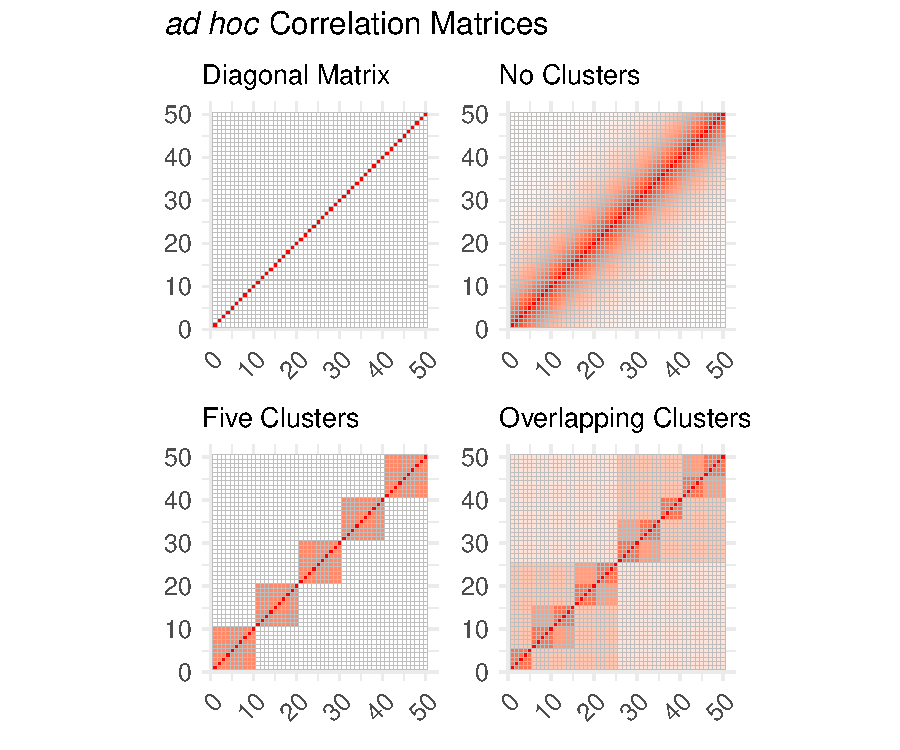
\includegraphics{Thesis_files/figure-latex/corr mats-1.pdf}
\caption{\label{corr_mats} Correlation Matricies}
\end{figure}

\hypertarget{emperical}{%
\subsubsection{\texorpdfstring{Emperical
\label{emp}}{Emperical }}\label{emperical}}

The empirical correlation matrix used in this study was calculated by
randomly selecting the daily returns for 50 of the largest (market
capitalization) 100, by market capitalization, S\&P 500 stocks between 1
January 2016 and 1 January 2021. The covariance matrix was then
calculated using the R package fitHeavyTail's fit\_mvt function. This
function uses ML estimation to fit a multivariate t-distribution to a
matrix of asset returns using to the following methodology.

Chuanhai Liu and Donald B. Rubin, ``ML estimation of the t-distribution
using EM and its extensions, ECM and ECME,'' Statistica Sinica (5),
pp.~19-39, 1995.

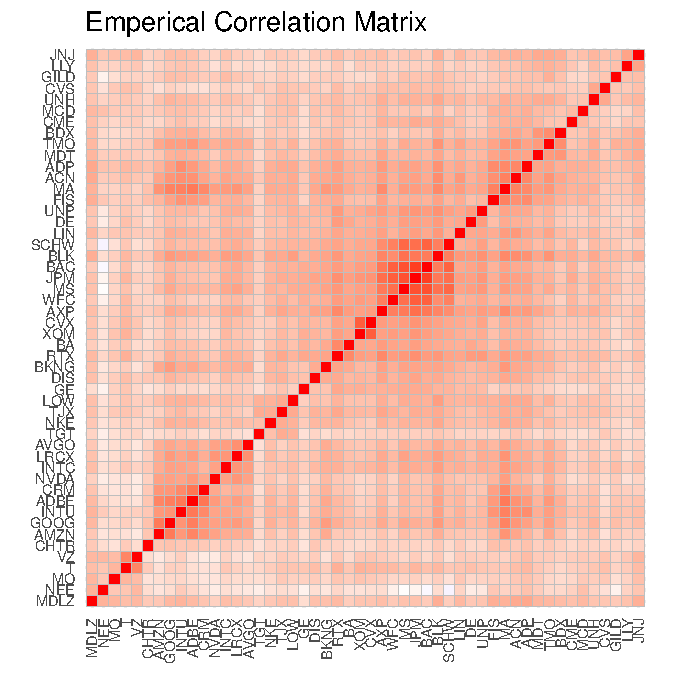
\includegraphics{Thesis_files/figure-latex/unnamed-chunk-1-1.pdf}

\hypertarget{eigen-values-and-condition-number}{%
\subsubsection{Eigen Values and Condition
Number}\label{eigen-values-and-condition-number}}

\hypertarget{monte-carlo}{%
\subsection{Monte Carlo}\label{monte-carlo}}

This work uses the R package MCmarket to carry out its Monte Carlo
simulations. This package uses a generalized Monte Carlo framework from
({\textbf{???}}).

\hypertarget{back-tests}. This additional
constraint is intended to prevent some portfolio's from building
excessively highly concentrated holdings, while remaining flexible
enough to punish those who do so. Therefore, the constraints are
effectively providing a fair playing ground for the portfolio's to
compete.

The first 50 periods were used to estimate the co-variance matrix, used
as the primary input in portfolio weight calculations for the respective
portfolios. These weights were then used in conjunction with the
simulated returns to calculate the returns for the respective
portfolios. d

\hypertarget{portfolio-analytics}{%
\subsection{Portfolio Analytics}\label{portfolio-analytics}}

\hypertarget{results-and-discussion}{%
\section{Results and Discussion}\label{results-and-discussion}}

\hypertarget{conclusion}{%
\section{Conclusion}\label{conclusion}}

I hope you find this template useful. Remember, stackoverflow is your
friend - use it to find answers to questions. Feel free to write me a
mail if you have any questions regarding the use of this package. To
cite this package, simply type citation(``Texevier'') in Rstudio to get
the citation for Katzke (\protect\hyperlink{ref-Texevier}{2017}) (Note
that united references in your bibtex file will not be included in
References).

\newpage

\hypertarget{references}{%
\section*{References}\label{references}}
\addcontentsline{toc}{section}{References}

\hypertarget{refs}{}
\leavevmode\hypertarget{ref-ardia2017}{}%
Ardia, D., Bolliger, G., Boudt, K. \& Gagnon-Fleury, J.-P. 2017. The
impact of covariance misspecification in risk-based portfolios.
\emph{Annals of Operations Research}. 254(1-2):1--16.

\leavevmode\hypertarget{ref-lopez2012}{}%
Bailey, D.H. \& Lopez De Prado, M. 2012. Balanced baskets: A new
approach to trading and hedging risks. \emph{Journal of Investment
Strategies (Risk Journals)}. 1(4).

\leavevmode\hypertarget{ref-choueifaty2008}{}%
Choueifaty, Y. \& Coignard, Y. 2008. Toward maximum diversification.
\emph{The Journal of Portfolio Management}. 35(1):40--51.

\leavevmode\hypertarget{ref-choueifaty2013}{}%
Choueifaty, Y., Froidure, T. \& Reynier, J. 2013. Properties of the most
diversified portfolio. \emph{Journal of investment strategies}.
2(2):49--70.

\leavevmode\hypertarget{ref-clarke2011}{}%
Clarke, R., De Silva, H. \& Thorley, S. 2011. Minimum-variance portfolio
composition. \emph{The Journal of Portfolio Management}. 37(2):31--45.

\leavevmode\hypertarget{ref-rawl2012}{}%
De Carvalho, R.L., Lu, X. \& Moulin, P. 2012a. Demystifying equity
risk--based strategies: A simple alpha plus beta description. \emph{The
Journal of Portfolio Management}. 38(3):56--70.

\leavevmode\hypertarget{ref-leote}{}%
De Carvalho, R.L., Lu, X. \& Moulin, P. 2012b. Demystifying equity
risk--based strategies: A simple alpha plus beta description. \emph{The
Journal of Portfolio Management}. 38(3):56--70.

\leavevmode\hypertarget{ref-demiguel2009}{}%
DeMiguel, V., Garlappi, L. \& Uppal, R. 2009. Optimal versus naive
diversification: How inefficient is the 1/n portfolio strategy?
\emph{The review of Financial studies}. 22(5):1915--1953.

\leavevmode\hypertarget{ref-lopez}{}%
De Prado, M.L. 2016. Building diversified portfolios that outperform out
of sample. \emph{The Journal of Portfolio Management}. 42(4):59--69.

\leavevmode\hypertarget{ref-fama1992}{}%
Fama, E.F. \& French, K.R. 1992. The cross-section of expected stock
returns. \emph{the Journal of Finance}. 47(2):427--465.

\leavevmode\hypertarget{ref-Texevier}{}%
Katzke, N.F. 2017. \emph{Texevier: Package to create elsevier templates
for rmarkdown}. ed. Stellenbosch, South Africa: Bureau for Economic
Research.

\leavevmode\hypertarget{ref-maillard2010}{}%
Maillard, T., Roncalli. 2010. The properties of equally weighted risk
contribution portfolios. \emph{The Journal of Portfolio Management}.
36(4):60--70.

\leavevmode\hypertarget{ref-markowitz}{}%
Markowitz, H. 1952. Portfolio selection. \emph{The Journal of Finance}.
7(1):77--91.

\leavevmode\hypertarget{ref-zhou2019}{}%
Zhou, R., Liu, J., Kumar, S. \& Palomar, D.P. 2019. Robust factor
analysis parameter estimation. In ed. Springer \emph{International
conference on computer aided systems theory}. 3--11.

\newpage

\hypertarget{appendix}{%
\section*{Appendix}\label{appendix}}
\addcontentsline{toc}{section}{Appendix}

\hypertarget{hierarchical-risk-parity-hrp}{%
\subsubsection{Hierarchical Risk Parity
(HRP)}\label{hierarchical-risk-parity-hrp}}

Due to the multitude of robustness issues related to traditional
portfolio optimisers, De Prado (\protect\hyperlink{ref-lopez}{2016})
developed a new approach incorporating machine-learning methods and
graph theory ({\textbf{???}}). De Prado
(\protect\hyperlink{ref-lopez}{2016}) argues that the ``lack of
hierarchical structure in a correlation matrix allows weights to vary
freely in unintended ways'' and that this contributes to the instability
issues. His HRP algorithm requires only a singular co-variance matrix
and can utilize the information within without the need for the positive
definite property (De Prado, \protect\hyperlink{ref-lopez}{2016}). This
procedure works in three stages:

De Prado (\protect\hyperlink{ref-lopez}{2016}) carried out an in sample
simulation study comparing the respective allocations of the long-only
minimum variance, IVP and HRP portfolios using a co-variance matrix
using a condition number that is ``not unfavourable'' to the minimum
variance portfolio. The simulated data consisted of 10000 observations
across 10 variables. The following findings were made: The minimum
variance portfolio concentrated 92.66\% of funds in the top 5 holdings
and assigned a zero weight to 3 assets. \emph{Conversly}, HRP only
assigned 62.5\% of its funds to the top 5 holdings (De Prado,
\protect\hyperlink{ref-lopez}{2016}). The minimum variance portfolio's
objective function causes it to build highly concentrated portfolio's in
favor of a small reduction in volatility; the HRP portfolio had only a
slightly higher volatility (De Prado,
\protect\hyperlink{ref-lopez}{2016}). This apparent diversification
advantage achieved by the minimum variance portfolio is rather deceptive
as the portfolio remains highly susceptible to idiosyncratic risk
incidents within its top holdings (De Prado,
\protect\hyperlink{ref-lopez}{2016}). This claim was further validated
by the finding that HRP achieved significantly lower out of sample
variance compared to the minimum variance portfolio. \#\# Appendix A
\{-\}

Some appendix information here

\hypertarget{appendix-b}{%
\subsection*{Appendix B}\label{appendix-b}}
\addcontentsline{toc}{subsection}{Appendix B}

\bibliography{Tex/ref}





\end{document}
